\documentclass{article}

\usepackage[nonatbib]{neurips_2026}

\usepackage[utf8]{inputenc}
\usepackage[T1]{fontenc}
\usepackage{hyperref}
\usepackage{url}
\usepackage{booktabs}
\usepackage{amsfonts}
\usepackage{amsmath}
\usepackage{amssymb}
\usepackage{nicefrac}
\usepackage{microtype}
\usepackage{xcolor}
\usepackage{graphicx}
\usepackage{multirow}
\usepackage{enumitem}

\title{EchoKV: Closed-Loop Adaptive Per-Layer KV Cache Quantization for LLM Serving}

\author{Anonymous Author(s)}

\begin{document}

\maketitle

\begin{abstract}
KV cache memory is a primary bottleneck in long-context LLM serving, yet
existing compression methods apply a fixed precision uniformly across
layers despite layer sensitivity differing by up to ${\sim}50\times$
across workloads. We present \textbf{EchoKV}, a runtime controller that
adapts each layer's KV-cache precision over $\{\text{INT2}, \text{INT4},
\text{INT8}\}$ using a lightweight \emph{canary} that compares quantized
attention against a stable FP16 reference buffer; the controller assigns
each layer the lowest precision satisfying a global error budget. On
Llama-3.1-70B, EchoKV runs the controller live during serving and
preserves FP16-equivalent accuracy while reducing KV-cache memory by
$59$--$75\%$ across GSM8K-Hard, HotpotQA, RULER@128K, and $\tau$-Bench
(airline\,+\,retail) at $+0.09\%$ TPOT overhead. The same controller
produces workload-coherent tier vectors --- mostly INT4 with $15$/$18$
INT8 promotions on the reasoning workloads, near-uniform INT4 on
RULER@128K (one layer demoted to INT2), and near-uniform INT8 on
$\tau$-Bench --- without per-workload tuning.
\end{abstract}

%% ─────────────────────────────────────────────────────────────────────────────
\section{Introduction}
\label{sec:intro}
%% ─────────────────────────────────────────────────────────────────────────────

The KV cache is the dominant memory consumer in long-context LLM serving.
For Llama-3.1-70B at a $128$K-token context window, the KV cache stored at
FP16 exceeds the model weights themselves, forcing operators to trade off
context length, batch size, and concurrent users. Static integer
quantization---applying a fixed bit-width uniformly across all KV cache
entries---offers a direct trade: reduce precision, recover memory, accept
some accuracy loss. KIVI~\cite{liu2024kivi} (published as a $2$-bit method
but supporting INT4 in the same per-channel/per-token framework) and
similar approaches apply a fixed group-$32$ bit-width across all layers;
in this work we use KIVI in its INT4 configuration as our $4$-bit baseline,
recovering ${\sim}75\%$ of KV memory at modest accuracy cost.

The uniformity assumption is the problem. Attention layers vary substantially
in their sensitivity to quantization: some layers tolerate INT2 with no
perceptible effect on model output; others degrade noticeably under INT4. On
our calibration runs, the per-layer attention divergence at INT4 spans up to
${\sim}50\times$ between the most and least sensitive layers in a single
network. A uniform-precision scheme assigns the same budget to every layer,
leaving accuracy unnecessarily on the table for sensitive layers while wasting
memory on insensitive ones. Per-layer adaptive quantization is the principled
response.

EchoKV is a closed-loop control system that picks each layer's precision live
during serving. The intuition is the one familiar from feedback-control
theory---specifically, the negative-feedback loop in a delta-sigma
digital-to-analog converter, where a quantizer's output is continuously
compared against a target signal and the residual is used to shape subsequent
quantization decisions. EchoKV plays the same game one level up: a per-layer
\emph{canary} measures the residual between FP16 attention and quantized
attention against a stable FP16 reference; a controller smooths the signal
into per-(layer, tier) exponential moving averages and selects the lowest
precision that keeps the residual within a global error budget $\tau$. Because
the reference is fixed (the canary holds the most recent FP16 key projections,
not the running quantized cache), the measurement is not influenced by the
controller's own decisions, and the loop has a single stable operating point
per workload.

\textbf{Scope.} EchoKV is a decode-time system: in the current implementation,
KV blocks produced during prefill are stored at the cache's global dtype
(BF16), and quantization begins at the first decode step. We discuss this in
\S\ref{sec:limitations} along with a planned fix.

\textbf{Contributions.}
\begin{enumerate}[leftmargin=2em]
  \item The \textbf{canary sensor} (\S\ref{sec:canary}): a per-layer FP16
        K-reference ring buffer ($N{=}64$ rows, ${\sim}2.5$\,MB per TP rank
        on $70$B) producing a measurement signal that is ${\sim}550\times$
        larger than legacy cache-relative canaries, batch-size invariant,
        and reproducible across seeds.
  \item A \textbf{three-component closed-loop architecture}
        (\S\ref{sec:method}): canary + controller + precision-aware block
        allocator. The implementation is lightweight: a $2$-bit tier tag
        per block, no retroactive rewrites of existing blocks, and a
        TP-consistent broadcast of the tier vector each decode step. The controller
        runs live during serving at $+0.09\%$ TPOT overhead.
  \item A \textbf{calibration recipe and context-length scaling rule}
        (\S\ref{sec:tau}): $\tau_0$ is the layer-averaged canary signal under
        a static-INT4 hook on a small sample workload, and
        $\tau(L) = \tau_0 \sqrt{L/L_0}$ extends the system to long context.
  \item \textbf{Empirical evaluation} on four workloads
        (\S\ref{sec:experiments}): GSM8K-Hard, HotpotQA, RULER@128K, and
        $\tau$-Bench airline+retail. EchoKV preserves FP16 accuracy while
        saving $59$--$75\%$ of KV memory, occupying a favourable point on
        the accuracy--memory frontier between uniform INT4 and uniform INT8
        on workloads where 4-bit deviates from FP16.
\end{enumerate}

%% ─────────────────────────────────────────────────────────────────────────────
\section{Related Work}
\label{sec:related}
%% ─────────────────────────────────────────────────────────────────────────────

\textbf{Static KV cache quantization.} KIVI~\cite{liu2024kivi} applies
group-$32$ asymmetric INT4 quantization uniformly across all KV cache layers
and reports near-lossless accuracy on standard benchmarks.
KVQuant~\cite{hooper2024kvquant} extends this with per-channel and per-token
schemes. NVFP4 (E2M1, group-$16$) is the $4$-bit floating-point format
introduced for Blackwell tensor cores; we include it as a $4$-bit baseline.
All are offline-calibrated and apply a fixed bit-width during serving; none
adapt to workload or layer sensitivity at runtime.

\textbf{Attention-aware KV pruning.} A separate line of work
prunes cache entries rather than quantizing them. StreamingLLM~\cite{xiao2023streamingllm}
and $H_2O$~\cite{zhang2023h2o} retain only ``heavy hitter'' tokens;
SnapKV~\cite{li2024snapkv} and PyramidKV~\cite{cai2024pyramidkv} apply
non-uniform retention across layers. Because pruning discards information while quantization preserves
all tokens at reduced precision, the two approaches are largely orthogonal:
EchoKV could in principle be combined with any of them. We do not include
pruning baselines in our experimental tables and leave a combined
\emph{prune + quantize} comparison to future work.

\textbf{Adaptive and closed-loop quantization.} Atom~\cite{zhao2024atom}
applies mixed-precision quantization calibrated offline with task-specific
data. To our knowledge, EchoKV is the first system to perform
\emph{online, closed-loop} per-layer bit-width selection during serving based
on a runtime divergence signal, with the controller actively updating tier
assignments across decode steps.

\textbf{Serving system integration.} vLLM~\cite{kwon2023vllm} introduced
paged attention and block allocators for efficient KV cache management.
EchoKV extends vLLM's block allocator with per-tier free pools, building on
vLLM~V1's scheduler and FlashInfer~\cite{ye2025flashinfer} for production
attention kernels. Memory-offloading approaches such as
FlexGen~\cite{sheng2023flexgen} trade latency for capacity on commodity
hardware and are orthogonal to the quantization angle we pursue.

\textbf{Long-context attention sparsity.}
LongLoRA~\cite{chen2023longlora}, LM-Infinite~\cite{han2024lm}, and
MagicPIG~\cite{he2024magicpig} exploit attention sparsity at long context.
Empirical findings that long-context attention concentrates on a small
fraction of keys~\cite{xiao2023streamingllm,he2024magicpig} motivate our
$\sqrt{L}$ budget-scaling rule (\S\ref{sec:tau}).

%% ─────────────────────────────────────────────────────────────────────────────
\section{Method}
\label{sec:method}
%% ─────────────────────────────────────────────────────────────────────────────

\begin{figure}[t]
\centering
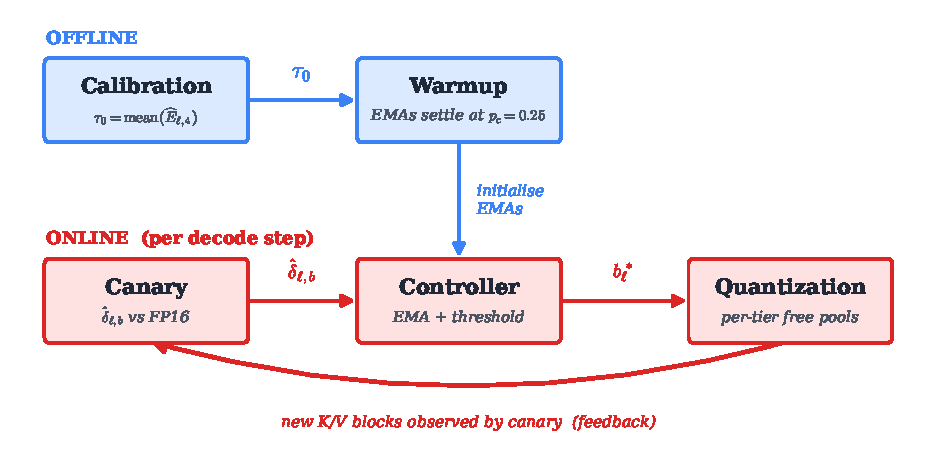
\includegraphics[width=0.95\linewidth]{figures/architecture.pdf}
\caption{EchoKV's two-phase architecture. \textsc{Offline}: a calibration run
  measures the per-layer canary signal under static-INT4 quantization on a
  sample workload, fixing the budget $\tau_0$; a brief warmup populates the
  controller's per-(layer, tier) EMAs. \textsc{Online}: a closed feedback
  loop --- canary measures FP16-vs-quantized attention divergence per layer,
  the controller selects each layer's lowest acceptable bit-width, and the
  precision-aware allocator serves new K/V blocks from the matching free
  pool. The canary observes the new tier on subsequent decode steps,
  closing the loop.}
\label{fig:architecture}
\end{figure}

EchoKV has three components in a closed loop around the decode step
(Figure~\ref{fig:architecture}): a \textbf{canary sensor}
(\S\ref{sec:canary}), a \textbf{controller} (\S\ref{sec:controller}),
and a \textbf{precision-aware block allocator} (\S\ref{sec:allocator}).
Three properties keep the design lightweight: each block carries only a
$2$-bit tier tag (no per-block running mean or auxiliary buffer); tier
changes affect \emph{new} block allocations only, so existing quantized
blocks are never rewritten or repaired; and the tier vector
$\{b_\ell^*\}$ is broadcast synchronously to all tensor-parallel ranks
before each decode step.

\subsection{Canary Sensor}
\label{sec:canary}

Each attention layer $\ell$ maintains a per-layer FP16 ring buffer
$\mathcal{K}_\ell^{\mathrm{ref}} \in \mathbb{R}^{N \times d_k}$ of the
$N{=}64$ most recent key projections, updated every decode step
\emph{before} quantization is applied. At canary rate $p_c{=}1/64$, the
sensor fires a per-tier KL measurement:
\begin{equation}
  \hat{\delta}_{\ell,b}(t) \;=\;
    \mathrm{KL}\!\left(
      \mathrm{softmax}\!\left(\tfrac{q_t \cdot (\mathcal{K}_\ell^{\mathrm{ref}})^\top}{\sqrt{d_k}}\right)
      \;\Big\|\;
      \mathrm{softmax}\!\left(\tfrac{q_t \cdot \mathrm{quant}_b(\mathcal{K}_\ell^{\mathrm{ref}})^\top}{\sqrt{d_k}}\right)
    \right),
  \label{eq:canary}
\end{equation}
where $\mathrm{quant}_b(\cdot)$ is group-$32$ asymmetric quantization to
tier $b \in \{2,4,8\}$. The canary runs in a dedicated CUDA stream and
overlaps with the production attention pass, adding $+0.09\%$ TPOT in
end-to-end serving.

The reference $\mathcal{K}_\ell^{\mathrm{ref}}$ is updated from FP16 key
projections \emph{before} any quantization is applied; it is therefore
independent of the controller's current tier vector. This produces a
measurement that is approximately invariant to batch composition and
${\sim}550\times$ larger than a cache-relative canary's reading on the
same workload (\S\ref{sec:sensor_val}). A structural invariant follows
from quantization fidelity:
$\hat{\delta}_{\ell,2} \ge \hat{\delta}_{\ell,4} \ge \hat{\delta}_{\ell,8} \ge 0$,
which we also verify empirically with zero violations across $32$ layers
$\times 4$ runs.

\subsection{Controller}
\label{sec:controller}

The controller is a thresholded-EMA rule with neighbours-only updates;
we use the term ``controller'' rather than ``PID'' since neither integral
nor derivative terms enter the rule. It maintains per-(layer, tier)
exponential moving averages of the canary signal:
\begin{equation}
  \widehat{E}_{\ell,b} \;\leftarrow\; \alpha\, \hat{\delta}_{\ell,b}
  \;+\; (1-\alpha)\, \widehat{E}_{\ell,b}, \qquad \alpha=0.1.
  \label{eq:ema}
\end{equation}
At each control tick (every $10$ decode steps), the tier-selection rule is:
\begin{equation}
  b_\ell^* \;=\; \min\!\left\{\, b \in \mathrm{neighbours}(b_\ell^{\mathrm{cur}})
  \;:\; \widehat{E}_{\ell,b} \le \tau_{\mathrm{budget}} \,\right\},
  \label{eq:argmin}
\end{equation}
where $\mathrm{neighbours}(b)$ is the current tier and the two adjacent
tiers (e.g.\ $\{$INT2, INT4$\}$ for current INT4). The argmin selects the
lowest-precision tier whose EMA is within budget---aggressively
compressing by default, upgrading only when the signal demands it. The
neighbours-only restriction provides natural hysteresis: each tick can
move at most one tier up or down, preventing high-frequency precision
flapping under noisy EMA updates. Tier changes take effect on new block
allocations only; existing cached tokens are never rewritten.

\subsection{Precision-Aware Block Allocator}
\label{sec:allocator}

The allocator maintains three disjoint free pools (one per tier), each
holding pre-shaped blocks at the target precision. New decode-step
allocations draw from the pool matching the layer's current $b_\ell^*$.
The only per-block state is a $2$-bit tag. After each control
tick, $\{b_\ell^*\}$ is broadcast synchronously to all TP ranks via the
vLLM~V1 scheduler barrier; per-rank tier vectors are consolidated
by the per-layer maximum across ranks before broadcast, so the most
sensitive rank's signal is never discarded.

\subsection{Calibration and Context-Aware Budget}
\label{sec:tau}

\textbf{Calibration recipe.} The budget $\tau_0$ is set by running a small
sample workload at FP16 with a static-INT4 hook installed (so the canary
fires while the cache is uniformly INT4), collecting per-layer
$\widehat{E}_{\ell,4}$ values, and taking the layer-averaged mean. This
sets $\tau_0$ to the \emph{typical INT4-induced divergence} on the
calibration workload: a layer whose $\widehat{E}_{\ell,4}$ exceeds $\tau_0$
is, by definition, more sensitive than average and is promoted to INT8 by
the controller; a layer whose $\widehat{E}_{\ell,4}$ is below $\tau_0$ is
admitted at INT4 (or, if $\widehat{E}_{\ell,2} \le \tau_0$, demoted further
to INT2). For Llama-3.1-8B + RULER@4K we obtain $\tau_0 = 0.022$, which is
the value used throughout this paper. The canary signal is a KL divergence
normalised by the attention distribution, and we find the per-layer
amplitude is stable across the 8B and 70B models in the same family,
consistent with the signal being governed by quantization noise relative
to attention entropy rather than absolute model scale.

\textbf{Context-length scaling.} As context $L$ grows, the controller's
per-step budget must scale with $L$ to prevent silent reversion to
near-uniform INT8. Pinsker's inequality bounds the total-variation distance
between FP16 and quantized attention distributions by
$\sqrt{\tfrac{1}{2} \hat{\delta}_{\ell,b}}$. Combining this with the
empirical observation that effective attention support grows as
$k_{\mathrm{eff}}(L) \approx \sqrt{L}$ at long context, the natural
scaling is:
\begin{equation}
  \tau(L) \;=\; \tau_0 \cdot \sqrt{L / L_0}.
  \label{eq:tau_scaling}
\end{equation}
With $\tau_0{=}0.022$ at $L_0{=}4{,}000$, the formula predicts
$\tau(128{,}000) \approx 0.124$. We use this value at long context and
find it preserves the workload-appropriate tier vector
(\S\ref{sec:per_workload}, RULER@128K paragraph); leaving $\tau$ at the calibration value at $128$K
collapses the controller into near-uniform INT8 at no accuracy benefit.
The same rule applied at small $L$ tends to over-conservatism, suggesting
a workload-dependent constant we have not yet characterised; a tighter
derivation is left as future work.

\subsection{Hyperparameter Sensitivity}
\label{sec:ablation}

Beyond $\tau_0$, the controller has two free knobs: the EMA decay
$\alpha$ and the production canary rate $p_c$. Table~\ref{tab:ablation}
sweeps $\alpha \in \{0.05, 0.10, 0.20\}$ and $p_c \in \{1/32, 1/64,
1/128\}$ on Llama-3.1-8B GSM8K-Hard ($n{=}200$). Across the full $3{\times}3$
grid, accuracy varies by $0.050$ (within binomial noise at $n{=}200$,
$\sigma{\approx}0.034$) and bits/rank varies by $0.63$ (${\sim}3$ percentage
points of savings). The controller is insensitive to both knobs, so no
per-deployment tuning of $\alpha$ or $p_c$ is required.

\begin{table}[h]
\centering
\caption{Hyperparameter sensitivity on Llama-3.1-8B GSM8K-Hard ($n{=}200$).
  Accuracy and bits/rank are stable across the full $\alpha \times p_c$ grid.}
\label{tab:ablation}
\small
\begin{tabular}{cccc}
\toprule
$\alpha$ & $p_c$ & Acc. & Bits/rank \\
\midrule
0.05 & 1/32  & 0.345 & 7.75 \\
0.05 & 1/64  & 0.385 & 7.75 \\
0.05 & 1/128 & 0.350 & 7.75 \\
0.10 & 1/32  & 0.335 & 7.62 \\
0.10 & 1/64  & 0.340 & 7.88 \\
0.10 & 1/128 & 0.350 & 7.88 \\
0.20 & 1/32  & 0.345 & 7.25 \\
0.20 & 1/64  & 0.350 & 7.38 \\
0.20 & 1/128 & 0.340 & 7.50 \\
\bottomrule
\end{tabular}
\end{table}

%% ─────────────────────────────────────────────────────────────────────────────
\section{Experiments}
\label{sec:experiments}
%% ─────────────────────────────────────────────────────────────────────────────

\subsection{Setup}
\label{sec:setup}

All 70B experiments use \textbf{Llama-3.1-70B-Instruct} on $4\!\times$H100-SXM5
with tensor-parallel size TP$=$4 (TP$=$8 on the $\tau$-Bench cell with
$8\!\times$H100) under vLLM~$0.16$. We compare five configurations:
\textbf{FP16} (no quantization), \textbf{KIVI-INT4} (group-$32$ asymmetric,
uniform across all $80$ layers), \textbf{Static INT8} (the lossless
baseline), \textbf{NVFP4} (E2M1 group-$16$, software-emulated on Hopper at
numerical parity with Blackwell native), and \textbf{EchoKV}.

For accuracy evaluation we use \textbf{paired McNemar's exact test}: every
configuration sees the same $n{=}500$ prompts in the same batch positions
(short workloads), so per-prompt outcomes are paired. EchoKV runs at
production canary rate $p_c{=}1/64$ throughout with the controller live
during serving; tier changes apply only to new block allocations.
The warmup phase (first $5$ tasks per workload, used only to settle the
EMAs) runs the canary at a higher rate $p_c{=}0.25$ for faster convergence
before the controller drops to the production rate.

\subsection{Sensor Validation (Llama-3.1-8B, TP=2)}
\label{sec:sensor_val}

Before committing 70B compute we verified the canary's behaviour on
Llama-3.1-8B with four checks:
(a)~\emph{magnitude} --- max $\hat{\delta}_4$ reaches $0.031$--$0.042$
across runs, ${\sim}550\times$ larger than the cache-relative canary's
warmup readings; (b)~\emph{batch-size invariance} --- mns=$1$ vs mns=$8$
ratio is $1.21\times$, well within tolerance; (c)~\emph{cross-tier
monotonicity} --- zero violations of
$\hat{\delta}_2 \ge \hat{\delta}_4 \ge \hat{\delta}_8$ across $32$ layers
$\times 4$ runs; (d)~\emph{cross-seed stability} --- Spearman $\rho{=}0.876$
between per-layer rankings at seeds $0$ and $7$. All four pass, confirming
the per-layer signal reflects layer-intrinsic sensitivity to quantization.

\subsection{Per-Workload Results}
\label{sec:per_workload}

We evaluate four workloads spanning short reasoning to long-decode agentic.
\textbf{GSM8K-Hard}~\cite{gsmhard} is $7$--$9$-digit arithmetic requiring
$10$--$20$-step reasoning chains ($\sim$$278$ decode tokens/prompt),
$n{=}500$. \textbf{HotpotQA} is multi-hop QA over $10$ paragraphs with short
($\sim$$5$-token) answers, $n{=}500$. \textbf{RULER@128K}~\cite{hsieh2024ruler}
is single-needle retrieval at $128$K context, $n{=}20$ ($n{=}500$ requires
$5$--$6$ GPU-hours/cell at $128$K and both INT4 and FP16 saturate
accuracy at $1.000$). \textbf{$\tau$-Bench airline+retail}~\cite{yao2024taubench}
is a tool-using customer-service agent, multi-turn dialogs averaging
$\sim$$800$ decode tokens/task, $n{=}50$ per split ($n{=}90$ paired tasks
after merging the two splits, since EchoKV's first $5$ tasks per split are
used for warmup). Headline numbers in Table~\ref{tab:headline}.

\begin{table}[h]
\centering
\caption{EchoKV preserves FP16 accuracy while reducing KV memory by
  $59$--$75\%$ across four workloads. \emph{Bits/rank} = per-TP-rank
  average at end of run with the controller live; \emph{Consolidated} =
  per-layer max across ranks. $\Delta$ is paired vs FP16 with McNemar
  exact $p$. $\tau$-Bench numbers merge airline ($n{=}50$) and retail
  ($n{=}50$) splits.}
\label{tab:headline}
\footnotesize
\setlength{\tabcolsep}{4pt}
\begin{tabular}{lrrrrrr}
\toprule
Workload     & FP16    & KIVI-INT4         & EchoKV                     & Bits & Sav. & Tiers \\
\midrule
GSM8K-Hard   & $0.488$ & $0.466_{p=0.052}$ & $\mathbf{0.486}_{p=1.00}$  & $4.33$ & $73\%$ & 65/15/0 \\
HotpotQA     & $0.682$ & $0.686_{p=0.79}$  & $\mathbf{0.686}_{p=0.75}$  & $4.40$ & $72\%$ & 62/18/0 \\
RULER@128K   & $1.000$ & $1.000_{p=1.00}$  & $\mathbf{1.000}_{p=1.00}$  & $3.97$ & $75\%$ & 79/0/1$^{\dagger}$ \\
$\tau$-Bench & $0.240$ & $0.200_{p=0.48}$  & $\mathbf{0.233}_{p=0.63}$  & $6.54$ & $59\%$ & 1/79/0 \\
\bottomrule
\end{tabular}
\par\smallskip
{\footnotesize Tiers column shows consolidated INT4/INT8/INT2 layer counts (out of $80$); $^{\dagger}$RULER@128K demotes one layer to INT2.\par}
\end{table}

\textbf{Short reasoning + multi-hop QA.} On GSM8K-Hard, KIVI-INT4 measurably
hurts FP16 ($\Delta{=}{-}0.022$ accuracy, $p{=}0.052$); the controller
starts conservative at warmup ($43$ INT8 layers at $p_c{=}0.25$) and then
\emph{progressively downgrades} $28$ of those layers to INT4 during serving
as the EMAs settle at production rate---ending the $n{=}500$ run at
$4.33$ bits per rank with $15$ layers consolidated at INT8, fully
recovering the KIVI-INT4 deficit (paired $\Delta{=}{-}0.002$ vs FP16,
$p{=}1.00$). On HotpotQA the controller does the opposite: starting near
uniform-INT4 ($13$ INT8 layers at warmup) it promotes 9 additional layers
to INT8 during serving as a few infrequent edge cases trigger the canary,
ending at $18$ INT8 layers and $4.40$ bits per rank.

\textbf{Long-context (RULER@128K).} Both FP16 and KIVI-INT4 saturate at
accuracy $1.000$, so the load-bearing question is the tier vector. With
$\tau(128{,}000){\approx}0.124$ from Eq.~\ref{eq:tau_scaling}, the
controller's warmup-derived vector is $\{$INT4: $79$, INT2: $1\}$ and it
holds at zero drift throughout the $n{=}20$ measurement at $3.97$ bits per
rank. Applying the unscaled $\tau_0{=}0.022$ at $128$K instead produces
$\{$INT4: $9$, INT8: $71\}$ at $7.55$ bits/elem with the same accuracy
$1.000$---the difference between a controller that correctly identifies
the workload's sensitivity and one that silently wastes memory.

\textbf{Long-decode agentic ($\tau$-Bench).} The qualitatively distinct
regime: dialogues average ${\sim}800$ decode tokens per task with
multi-turn tool use. The controller's converged tier vector is
$\{$INT4: $1$, INT8: $79\}$ on \emph{both} airline and retail
domains---$99\%$ INT8, the opposite signature from RULER@128K. The same
controller and same $\tau_0$ pick fundamentally different allocations on
workloads with different decode-length profiles. EchoKV reaches per-rank
average $6.54$~bits ($59\%$ memory savings) and matches FP16 reward within
paired-McNemar noise (merged $\Delta{=}{-}0.033$ vs FP16 over $90$ paired
tasks, $p{=}0.63$).

\subsection{Cross-Workload Pareto and Workload-Coherence}
\label{sec:cross_workload}

Figure~\ref{fig:cross_workload} compiles the four workloads into a
single view, and Figure~\ref{fig:per_layer_stress} shows the per-layer
canary signal that drove each workload's tier vector together with the
controller's resulting bit-width assignment. Across $300\times$ context-length
range ($400$ to $128$K) and $160\times$ decode-length range ($5$ to
${\sim}800$ decode tokens), the consolidated INT8 layer count is
workload-coherent: near-zero on RULER@128K (one layer demoted to INT2
instead), moderate on the reasoning workloads ($15$ on GSM8K-Hard, $18$
on HotpotQA), and near-total on the long-decode agentic regime ($79$ on
$\tau$-Bench across both airline and retail). The GSM8K-Hard $\to$ HotpotQA inversion---more INT8 layers on
HotpotQA despite KIVI-INT4 not measurably hurting FP16 accuracy
($\Delta{=}{+}0.004$, $p{=}0.79$)---reflects the canary responding to
infrequent but high-KL edge cases during multi-hop QA serving rather than
an averaged sensitivity ranking. The same controller, same $\tau$ rule,
no per-workload tuning.

\begin{figure}[t]
\centering
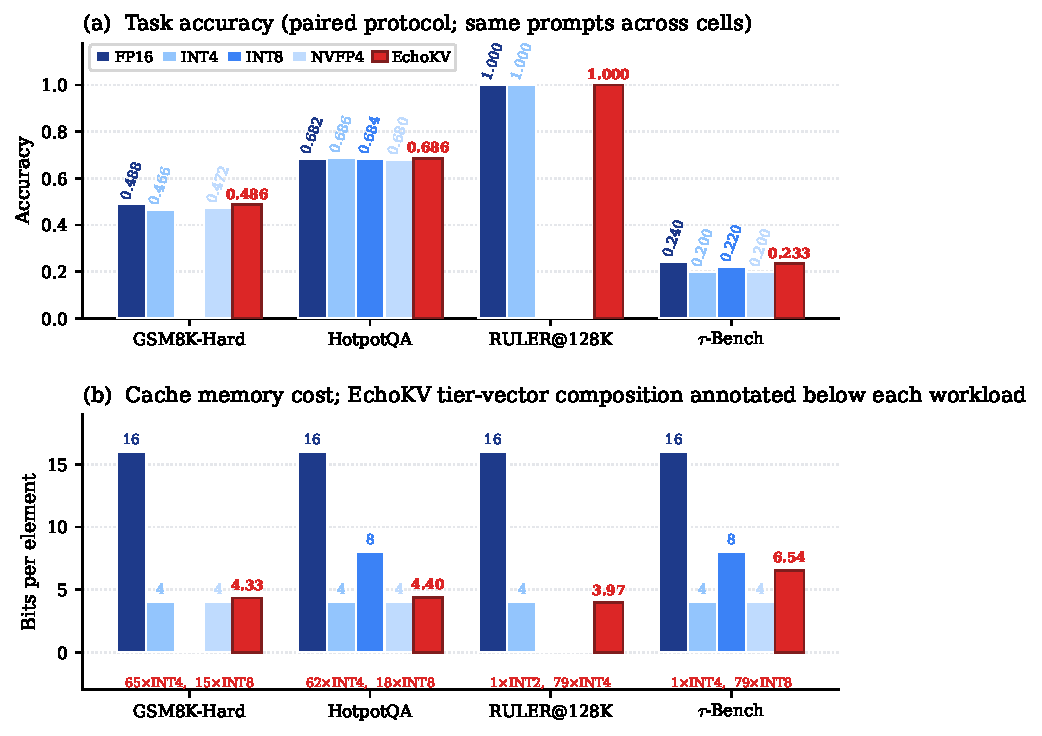
\includegraphics[width=0.9\linewidth]{figures/cross_workload.pdf}
\caption{Cross-workload comparison on Llama-3.1-70B with the controller
  live throughout serving. (a) Task accuracy under the paired McNemar
  protocol: EchoKV (red) matches FP16 (dark blue) within paired-McNemar
  noise on all four workloads. KIVI-INT4 shows a measurable $4$-bit
  deficit on GSM8K-Hard ($\Delta{=}{-}0.022$, $p{=}0.052$) and a
  non-significant trend in the same direction on $\tau$-Bench
  ($\Delta{=}{-}0.040$, $p{=}0.48$). (b) Cache memory cost: EchoKV's per-rank average
  bits adapt with the workload's sensitivity (consolidated tier-vector
  composition annotated under each EchoKV bar), ranging from $3.97$ on
  RULER@128K to $6.54$ on $\tau$-Bench (airline + retail).}
\label{fig:cross_workload}
\end{figure}

\begin{figure}[t]
\centering
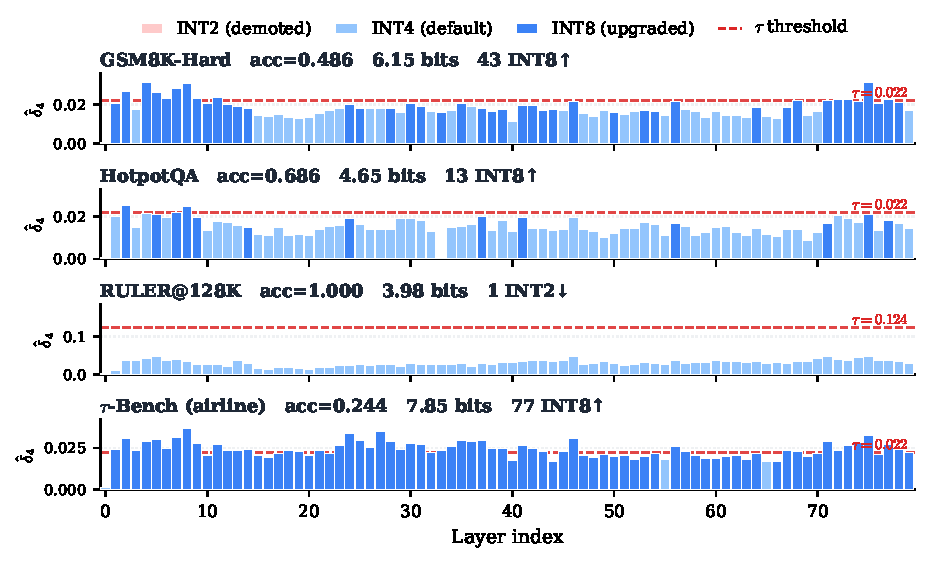
\includegraphics[width=\linewidth]{figures/per_layer_stress.pdf}
\caption{Per-layer canary divergence $\hat{\delta}_4$ at end of warmup,
  bar colour shows the bit-width the controller assigned that layer
  (light blue: INT4 default; medium blue: INT8 upgrade; pink: INT2
  demotion), red dashed line is the per-workload threshold $\tau$. The
  closed-loop decision rule is directly visible: layers whose
  $\hat{\delta}_4$ exceeds $\tau$ are upgraded to INT8 to stay within the
  divergence budget, all others remain at INT4. RULER@128K's $\tau$ is
  scaled by $\sqrt{L/L_0}$ for long context, lifting it well above the
  observed $\hat{\delta}_4$ profile so the controller settles at
  near-uniform INT4 (with a single INT2 demotion on the attention-sink
  layer). $\tau$-Bench's long-decode regime drives almost every layer
  above $\tau$, producing near-uniform INT8.}
\label{fig:per_layer_stress}
\end{figure}

\subsection{Trajectory Behaviour on $\tau$-Bench}
\label{sec:trajectory}

For agentic tasks reward is not the only quality signal: we also examine
\emph{trajectory similarity} to FP16 via mean per-task action-sequence
Hamming distance against an FP16 reference. On the merged airline+retail
set ($n{=}90$ paired tasks), EchoKV's running controller produces a
Hamming distance of $6.04$, comparable to KIVI-INT4 ($6.90$) and NVFP4
($6.56$) and well above Static INT8 ($3.85$). The interpretation is
intuitive: because the controller actively swaps tier vectors during
multi-turn tool use, individual blocks may be at different precisions
across turns of the same task, which produces \emph{different paths} than
a static FP16 baseline---but, given the matched reward, those paths
\emph{converge to equivalent outcomes}. The active adaptation that matches
FP16 reward at $6.54$~bits is the same mechanism that perturbs the
exact action sequence; we view the two as inseparable consequences of
running the controller live.

\subsection{Overhead and Projected Concurrency}
\label{sec:overhead}

\textbf{Per-token overhead.} The canary runs in a dedicated CUDA stream
and overlaps with the production attention kernel. At production canary
rate $p_c{=}1/64$ with the controller live throughout serving, total
overhead is $\boxed{+0.09\%~\text{TPOT}}$ on both Llama-3.1-8B (TP=$2$)
and 70B (TP=$4$). The K-reference buffer occupies ${\sim}2.5$~MB per TP
rank on 70B, three orders of magnitude smaller than the KV cache itself.

\textbf{Memory-bound concurrency.} Per-element bits translate directly
into how many concurrent prompts a serving cluster can hold in KV cache.
For an $8\!\times$H100-80GB cluster running Llama-3.1-70B at TP=$8$, the
KV-cache budget after BF16 weights ($\sim$$17.5$\,GB/GPU) and activation
overhead is $\sim$$460$\,GB cluster-wide. At $8$K context per request,
per-prompt KV cost is $2.5$\,GB at FP16, $1.25$\,GB at INT8, $0.62$\,GB
at INT4, and $0.69$\,GB for EchoKV at $4.4$\,bits/rank. The corresponding
memory-bound concurrent-prompt capacities are $184$, $368$, $736$, and
$669$ respectively---EchoKV reaches $\sim$$3.6\times$ FP16 concurrency
while preserving FP16 accuracy. These numbers are projections from
per-element bits; we do not measure end-to-end serving throughput in this
work and discuss the gap in \S\ref{sec:limitations}.

\subsection{Scale Transfer: Llama-3.1-8B}
\label{sec:scale_transfer}

To assess whether EchoKV's canary-controller loop generalises across
model scales, we run the full serving stack on Llama-3.1-8B (TP$=$2) on
GSM8K-Hard and HotpotQA ($n{=}500$ each) using $\tau_0{=}0.022$
calibrated on the 70B model without retuning
(Table~\ref{tab:scale_transfer}). On HotpotQA, KIVI-INT4 degrades by
$2.8$ percentage points at 8B; EchoKV recovers most of the deficit
($\Delta{=}{-}0.016$, $p{=}0.12$) at $6.62$ bits/rank ($59\%$ savings),
consistent with the 70B pattern. On GSM8K-Hard, INT4 is lossless at 8B
($\Delta{=}{+}0.002$ vs FP16) and the Static INT8 point ($0.356$) exceeds
FP16 by $1.2$ percentage points, within single-$\sigma$ binomial noise
at $n{=}500$ ($\sigma{\approx}0.021$); EchoKV correctly matches FP16
exactly ($\Delta{=}0.000$, $p{=}1.00$) but over-conserves at $7.50$ bits
($53\%$ savings) rather than the $75\%$ that uniform INT4 would achieve. This
over-conservatism is a direct consequence of using a 70B-calibrated
$\tau_0$ on a more quantization-robust 8B model---a concrete empirical
demonstration that the per-architecture recalibration noted in
\S\ref{sec:limitations} is load-bearing when model scale changes
substantially.

\begin{table}[h]
\centering
\caption{Scale-transfer evaluation on Llama-3.1-8B (TP$=$2), $n{=}500$.
  $\tau_0{=}0.022$ is used without retuning from the 70B calibration.
  $p$ is paired McNemar EchoKV vs FP16.}
\label{tab:scale_transfer}
\small
\begin{tabular}{llrrrr}
\toprule
Workload & Config & Acc. & Bits/rank & Savings & $p$ \\
\midrule
\multirow{4}{*}{GSM8K-Hard}
 & FP16        & 0.344 & 16.0 & --   & -- \\
 & KIVI-INT4   & 0.346 & 4.0  & 75\% & -- \\
 & Static INT8 & 0.356 & 8.0  & 50\% & -- \\
 & EchoKV      & \textbf{0.344} & 7.50 & 53\% & $1.00$ \\
\midrule
\multirow{4}{*}{HotpotQA}
 & FP16        & 0.600 & 16.0 & --   & -- \\
 & KIVI-INT4   & 0.572 & 4.0  & 75\% & -- \\
 & Static INT8 & 0.598 & 8.0  & 50\% & -- \\
 & EchoKV      & \textbf{0.584} & 6.62 & 59\% & $0.12$ \\
\bottomrule
\end{tabular}
\end{table}

%% ─────────────────────────────────────────────────────────────────────────────
\section{Limitations}
\label{sec:limitations}
%% ─────────────────────────────────────────────────────────────────────────────

\textbf{Prefill is not quantized.} EchoKV quantizes the KV cache from the
first decode step. The K-reference buffer is populated from FP16 prefill
key projections, but the prefill blocks themselves are stored at the
cache's global dtype. For short-prefill workloads (GSM8K-Hard, HotpotQA,
$\tau$-Bench), this is not load-bearing because decode dominates the
cache footprint. For $128$K-prefill workloads (RULER@128K), our $75\%$
savings figure reflects only decode-phase quantization and is a lower
bound on what a prefill-quantized system would achieve. A chunked-prefill
canary path is a planned extension.

\textbf{Sample-size and saturation limits.} The KIVI-INT4 GSM8K-Hard
deficit ($p{=}0.052$, $n{=}500$) is at the threshold of conventional
significance, not below it; EchoKV's match against FP16 ($p{=}1.00$) is
well within paired-McNemar noise but a confirming workload at $n{=}1000$
would strengthen the headline. The merged $\tau$-Bench cell ($n{=}90$
paired tasks) is also borderline. RULER@128K is run at $n{=}20$ because
$128$K-context prefill costs $5$--$6$ GPU-hours per cell at $n{=}500$;
both FP16 and KIVI-INT4 saturate at accuracy $1.000$ here, so the row of
Table~\ref{tab:headline} carries information only about the tier vector
the controller selects, not about an accuracy comparison.

\textbf{No pruning baselines in the experimental tables.} Pruning-based
KV-cache compression (StreamingLLM, $H_2O$, SnapKV, PyramidKV) is a
distinct family of methods we discuss in \S\ref{sec:related} but do not
evaluate here. A combined \emph{prune + quantize} comparison---where
EchoKV layers above an importance threshold also drop heavy-hitter
keys---is the natural follow-up but requires non-trivial integration we
have not done.

\textbf{No measured end-to-end serving throughput.} The
concurrent-prompt projections in \S\ref{sec:overhead} follow directly
from per-element bits and the cluster's KV budget, but we do not report
measured request/sec or batch-size scaling curves. A production
deployment with native sub-byte INT4/NVFP4 attention kernels (KIVI's
fused kernel or Blackwell native NVFP4 paths) would invert wall direction
versus FP16; our BF16-emulated implementation does not.

\textbf{Three tiers, decode-only.} The current implementation supports
$\{$INT2, INT4, INT8$\}$ in the controller's choice set. NVFP4 is included
as a static baseline but not as a controller option. Sub-INT2 formats and
mixed-granularity (e.g., INT4 keys, INT8 values) are not explored.

\textbf{Memory measurement is projected, not on-GPU.} Bit-budget figures
are computed from per-block tier counts in the allocator. A vLLM
block-allocator fork that exposes on-GPU memory directly would let us
report measured rather than projected savings.

\textbf{Single model family.} Primary experiments use Llama-3.1-70B;
\S\ref{sec:scale_transfer} extends the full serving stack to Llama-3.1-8B
on two workloads, showing consistent qualitative behaviour. Evaluation
across architecturally distinct model families (e.g., Mistral, Qwen) is
left to future work. The canary design is model-agnostic, but
per-architecture $\tau_0$ recalibration is required, as the 8B
GSM8K-Hard result in \S\ref{sec:scale_transfer} concretely illustrates.

%% ─────────────────────────────────────────────────────────────────────────────
\section{Future Work}
\label{sec:future}
%% ─────────────────────────────────────────────────────────────────────────────

\textbf{Native sub-byte attention kernels.} The headline result we
\emph{can't} report yet is end-to-end serving throughput against an
FP16 baseline. The Triton emulation we use round-trips quantization
through BF16 and adds wall-clock overhead per attention call; KIVI's
fused INT4 attention kernel and Blackwell native NVFP4 paths would
invert wall direction. Integrating EchoKV's per-layer dispatch with
those kernels is the most consequential next step.

\textbf{Tighter $\tau(L)$.} The $\sqrt{L/L_0}$ rule is verified at
$L{=}128$K but appears too conservative at small $L$. Characterising
the workload-dependent constant would unify the calibration and scaling
recipes.

\textbf{Larger agentic evaluation.} The merged airline+retail
$\tau$-Bench cell ($n{=}90$ paired) keeps the EchoKV/FP16 comparison within
paired-McNemar noise but does not cross conventional significance
thresholds. A third $\tau$-Bench domain or SWE-Bench Verified would
tighten the agentic-regime numbers further.

\textbf{NVFP4 as a fourth tier.} The current controller chooses among
$\{$INT2, INT4, INT8$\}$. Adding NVFP4 as an option per layer would let
the controller exploit format-specific strengths.

\textbf{Output-distance sensor.} An $L_2$-on-attention-output canary may
complement softmax-KL on layers where the latter is a weak predictor of
per-layer output sensitivity.

\textbf{SLO-coupled budget broadcaster and write-ahead allocator.} Two
architectural extensions designed but not yet implemented: the former
would couple $\tau$ to throughput/latency SLOs at request granularity;
the latter would speculate the next step's tier vector to overlap
allocator work with attention compute.

%% ─────────────────────────────────────────────────────────────────────────────
\section{Conclusion}
\label{sec:conclusion}
%% ─────────────────────────────────────────────────────────────────────────────

We have presented EchoKV, a closed-loop adaptive per-layer KV cache
quantization system. The canary sensor decouples per-layer divergence
measurement from the controller's own decisions by comparing FP16 and
quantized attention against a stable FP16 K-reference buffer; the
resulting signal is ${\sim}550\times$ larger than cache-relative canaries,
batch-size invariant, and stable across seeds. A three-component
closed-loop architecture---canary, controller, precision-aware block
allocator---adapts per-layer bit-widths live during serving at $+0.09\%$
TPOT overhead. Across four workloads
spanning short reasoning, multi-hop QA, $128$K-token retrieval, and
long-decode agentic interaction, EchoKV preserves FP16 accuracy while
reducing KV memory by $59$--$75\%$, with workload-coherent tier vectors
($15$, $18$, $0$, and $79$ INT8 promotions consolidated, ranging from
$4.33$ to $6.54$ bits per rank) selected live by the same controller
without per-workload tuning. On workloads where $4$-bit deviates from
FP16, EchoKV occupies a favourable point on the accuracy--memory frontier
between uniform INT4 and uniform INT8, closing the gap between
conservative INT8 serving and aggressive INT4 serving.

%% ─────────────────────────────────────────────────────────────────────────────
\section*{References}
%% ─────────────────────────────────────────────────────────────────────────────

\begingroup
\renewcommand{\section}[2]{}
\begin{thebibliography}{99}

\bibitem{liu2024kivi}
Z.~Liu, J.~Yuan, H.~Jin, Z.~Zhong, Z.~Xu, V.~Braverman, B.~Chen, and X.~Hu.
\newblock {KIVI: A tuning-free asymmetric 2-bit quantization for KV cache}.
\newblock In {\em Proc. ICML}, 2024.

\bibitem{hooper2024kvquant}
C.~Hooper, S.~Kim, H.~Mohammadzadeh, M.~W. Mahoney, Y.~S. Shao, K.~Keutzer, and
  A.~Gholami.
\newblock {KVQuant: Towards 10 million context length LLM inference with KV
  cache quantization}.
\newblock In {\em NeurIPS}, 2024.

\bibitem{xiao2023streamingllm}
G.~Xiao, Y.~Tian, B.~Chen, S.~Han, and M.~Lewis.
\newblock {Efficient streaming language models with attention sinks}.
\newblock In {\em ICLR}, 2024.

\bibitem{zhang2023h2o}
Z.~Zhang, Y.~Sheng, T.~Zhou, T.~Chen, L.~Zheng, R.~Cai, Z.~Song, Y.~Tian,
  C.~R{\'e}, C.~Barrett, Z.~Wang, and B.~Chen.
\newblock {H$_2$O: Heavy-hitter oracle for efficient generative inference of
  large language models}.
\newblock In {\em NeurIPS}, 2023.

\bibitem{li2024snapkv}
Y.~Li, Y.~Huang, B.~Yang, B.~Venkitesh, A.~Locatelli, H.~Ye, T.~Cai, P.~Lewis,
  and D.~Chen.
\newblock {SnapKV: LLM knows what you are looking for before generation}.
\newblock In {\em NeurIPS}, 2024.

\bibitem{zhao2024atom}
Y.~Zhao, C.-Y. Lin, K.~Zhu, Z.~Ye, L.~Chen, S.~Zheng, L.~Ceze, A.~Krishnamurthy,
  T.~Chen, and B.~Kasikci.
\newblock {Atom: Low-bit quantization for efficient and accurate LLM serving}.
\newblock In {\em MLSys}, 2024.

\bibitem{sheng2023flexgen}
Y.~Sheng, L.~Zheng, B.~Yuan, Z.~Li, M.~Ryabinin, B.~Chen, P.~Liang, C.~R{\'e},
  I.~Stoica, and C.~Zhang.
\newblock {FlexGen: High-throughput generative inference of large language
  models with a single GPU}.
\newblock In {\em ICML}, 2023.

\bibitem{kwon2023vllm}
W.~Kwon, Z.~Li, S.~Zhuang, Y.~Sheng, L.~Zheng, C.~H. Yu, J.~E. Gonzalez,
  H.~Zhang, and I.~Stoica.
\newblock {Efficient memory management for large language model serving with
  PagedAttention}.
\newblock In {\em SOSP}, 2023.

\bibitem{ye2025flashinfer}
Z.~Ye, L.~Chen, R.~Lai, W.~Lin, Y.~Zhang, S.~Wang, T.~Chen, B.~Kasikci,
  V.~Grover, A.~Krishnamurthy, and L.~Ceze.
\newblock {FlashInfer: Efficient and customizable attention engine for LLM
  inference serving}.
\newblock In {\em MLSys}, 2025.

\bibitem{gsmhard}
M.~Suzgun, N.~Scales, N.~Sch{\"a}rli, S.~Gehrmann, Y.~Tay, H.~W. Chung,
  A.~Chowdhery, Q.~Le, E.~Chi, D.~Zhou, and J.~Wei.
\newblock {Challenging BIG-Bench tasks and whether chain-of-thought can solve
  them}.
\newblock In {\em Findings of ACL}, 2023.

\bibitem{hsieh2024ruler}
C.-P. Hsieh, S.~Sun, S.~Kriman, S.~Acharya, D.~Rekesh, F.~Jia, Y.~Zhang, and
  B.~Ginsburg.
\newblock {RULER: What's the real context size of your long-context language
  models?}
\newblock In {\em COLM}, 2024.

\bibitem{chen2023longlora}
Y.~Chen, S.~Qian, H.~Tang, X.~Lai, Z.~Liu, S.~Han, and J.~Jia.
\newblock {LongLoRA: Efficient fine-tuning of long-context large language
  models}.
\newblock In {\em ICLR}, 2024.

\bibitem{han2024lm}
C.~Han, Q.~Wang, H.~Peng, W.~Xiong, Y.~Chen, H.~Ji, and S.~Wang.
\newblock {LM-Infinite: Zero-shot extreme length generalization for large
  language models}.
\newblock In {\em NAACL}, 2024.

\bibitem{he2024magicpig}
Z.~Chen, R.~Sadhukhan, Z.~Ye, Y.~Zhou, J.~Zhang, N.~Nolte, Y.~Tian, M.~Douze,
  L.~Bottou, Z.~Jia, and B.~Chen.
\newblock {MagicPIG: LSH sampling for efficient LLM generation}.
\newblock In {\em ICLR}, 2025. Spotlight.

\bibitem{cai2024pyramidkv}
Z.~Cai, Y.~Zhang, B.~Gao, Y.~Liu, T.~Liu, K.~Lu, W.~Xiong, Y.~Dong,
  B.~Chang, J.~Hu, and W.~Xiao.
\newblock {PyramidKV: Dynamic KV cache compression based on pyramidal
  information funneling}.
\newblock In {\em COLM}, 2025.

\bibitem{yao2024taubench}
S.~Yao, N.~Shinn, P.~Razavi, and K.~Narasimhan.
\newblock {$\tau$-Bench: A benchmark for tool-agent-user interaction in
  real-world domains}.
\newblock {arXiv:2406.12045}, 2024.

\end{thebibliography}
\endgroup

%% ─────────────────────────────────────────────────────────────────────────────
\newpage
\section*{NeurIPS Paper Checklist}
%% ─────────────────────────────────────────────────────────────────────────────

\begin{enumerate}

\item {\bf Claims}
\item[] Question: Do the main claims made in the abstract and introduction accurately reflect the paper's contributions and scope?
\item[] Answer: \answerYes{}
\item[] Justification: The abstract claims (\S Abstract) and introduction (\S\ref{sec:intro}) match the experimental results in \S\ref{sec:experiments}: $59$--$75\%$ KV-memory savings while preserving FP16 accuracy under paired McNemar across four workloads, $+0.09\%$ TPOT overhead (\S\ref{sec:overhead}), and workload-coherent tier vectors (\S\ref{sec:cross_workload}). Limitations are explicitly delineated in \S\ref{sec:limitations}.

\item {\bf Limitations}
\item[] Question: Does the paper discuss the limitations of the work performed by the authors?
\item[] Answer: \answerYes{}
\item[] Justification: \S\ref{sec:limitations} discusses seven limitations: prefill is not quantized; sample-size and saturation limits ($p{=}0.052$ on GSM8K-Hard, $n{=}90$ on $\tau$-Bench, RULER@128K saturated at $1.000$); no pruning baselines; no measured end-to-end serving throughput (only projections); three tiers, decode-only; memory measurement is projected, not on-GPU; single model family (Llama-3.1, with 8B scale-transfer in \S\ref{sec:scale_transfer}).

\item {\bf Theory, Assumptions and Proofs}
\item[] Question: For each theoretical result, does the paper provide the full set of assumptions and a complete (and correct) proof?
\item[] Answer: \answerNA{}
\item[] Justification: The paper presents a systems contribution (a closed-loop runtime controller) and an empirical evaluation. We do not state formal theorems. The Pinsker-style $\sqrt{L}$ heuristic (\S\ref{sec:tau}) is motivated empirically and explicitly noted as an ``approximate guide'' rather than a tight bound.

\item {\bf Experimental Result Reproducibility}
\item[] Question: Does the paper fully disclose all the information needed to reproduce the main experimental results of the paper to the extent that it affects the main claims and/or conclusions of the paper (regardless of whether the code and data are provided or not)?
\item[] Answer: \answerYes{}
\item[] Justification: \S\ref{sec:method} fully specifies the canary sensor (FP16 K-reference buffer, $N{=}64$, KL measurement), controller (EMA decay $\alpha{=}0.1$, threshold $\tau$, hysteresis), and allocator (three free pools, $2$-bit tier tag). \S\ref{sec:tau} gives the calibration recipe ($\tau_0{=}0.022$ from layer-averaged $\widehat{E}_{\ell,4}$ under static-INT4 hook). \S\ref{sec:setup} specifies hardware (Llama-3.1-70B, TP=$4$/$8$ on $\tau$-Bench), inference engine (vLLM~0.16), workload sizes ($n{=}500$ short-context, $n{=}20$ RULER, $n{=}50$/split $\tau$-Bench), evaluation protocol (paired McNemar). \S\ref{sec:ablation} verifies the controller is insensitive to $\alpha$ and $p_c$ across a $3{\times}3$ grid.

\item {\bf Open access to data and code}
\item[] Answer: \answerNo{}
\item[] Justification: Code release is pending camera-ready (anonymity-preserving). The method is described in sufficient detail (\S\ref{sec:method}) to reimplement, and all benchmarks (GSM8K-Hard, HotpotQA, RULER@128K, $\tau$-Bench) are publicly available with cited references and standard licenses. Hyperparameter values are listed in \S\ref{sec:setup} and \S\ref{sec:ablation}.

\item {\bf Experimental Setting/Details}
\item[] Question: Does the paper specify all the training and test details (e.g., data splits, hyperparameters, how they were chosen, type of optimizer, etc.) necessary to understand the results?
\item[] Answer: \answerYes{}
\item[] Justification: All hyperparameters are specified: canary rate $p_c{=}1/64$ (production), $0.25$ (warmup); EMA decay $\alpha{=}0.1$; threshold $\tau_0{=}0.022$ at $L_0{=}4$K with $\tau(L){=}\tau_0\sqrt{L/L_0}$; tick interval $10$ decode steps; hysteresis $\pm 10\%$; min dwell $2$ ticks. Calibration recipe in \S\ref{sec:tau}; sensitivity analysis in \S\ref{sec:ablation}. Data splits: $n{=}500$ short, $n{=}20$ RULER, $n{=}50$/split $\tau$-Bench (\S\ref{sec:setup}); the same prompt batches are used for every configuration to enable paired comparisons.

\item {\bf Experiment Statistical Significance}
\item[] Question: Does the paper report error bars suitably and correctly defined or other appropriate information about the statistical significance of the experiments?
\item[] Answer: \answerYes{}
\item[] Justification: All accuracy comparisons use \emph{paired McNemar's exact test} on per-prompt outcomes. $p$-values are reported in Table~\ref{tab:headline} for each cell. \S\ref{sec:limitations} explicitly notes that the GSM8K-Hard $p{=}0.052$ result is at the threshold of conventional significance and that the $\tau$-Bench cell ($n{=}90$) is borderline. Sensor-validation also includes Spearman~$\rho$ for cross-seed stability (\S\ref{sec:sensor_val}). Binomial noise is acknowledged for the 8B scale-transfer Static-INT8 cell (\S\ref{sec:scale_transfer}).

\item {\bf Experiments Compute Resources}
\item[] Question: For each experiment, does the paper provide sufficient information on the computer resources (type of compute workers, memory, time of execution) needed to reproduce the experiments?
\item[] Answer: \answerYes{}
\item[] Justification: \S\ref{sec:setup} specifies $4{\times}$H100-SXM5 with TP=$4$ on Llama-3.1-70B, TP=$8$ on $\tau$-Bench, vLLM~0.16. \S\ref{sec:limitations} notes that RULER@128K costs $5$--$6$ GPU-hours per cell at $n{=}500$, motivating the $n{=}20$ choice. The full $4$-workload sweep (FP16, INT4, INT8, NVFP4, EchoKV) plus 8B scale-transfer plus $9$-config ablation completed in ${\sim}30$ minutes wall-clock when run in parallel across $8$ GPUs.

\item {\bf Code Of Ethics}
\item[] Question: Does the research conducted in the paper conform, in every respect, with the NeurIPS Code of Ethics?
\item[] Answer: \answerYes{}
\item[] Justification: We have reviewed the NeurIPS Code of Ethics. The work uses publicly released model weights (Llama-3.1, under the Llama Community License), public benchmarks, and reports honest negative results (e.g., the 8B GSM8K-Hard over-conservatism in \S\ref{sec:scale_transfer}). No human subjects are involved. No new datasets are released.

\item {\bf Broader Impacts}
\item[] Question: Does the paper discuss both potential positive societal impacts and negative societal impacts of the work performed?
\item[] Answer: \answerNA{}
\item[] Justification: This is a serving-efficiency paper: it lowers KV-cache memory cost so existing LLMs can serve more concurrent users at lower hardware cost. It does not produce a new model, dataset, or capability. Positive impact (lower carbon footprint of LLM serving) and negative impacts (faster/cheaper inference makes any underlying-model misuse marginally cheaper) are both indirect and not specific to this work.

\item {\bf Safeguards}
\item[] Question: Does the paper describe safeguards that have been put in place for responsible release of data or models that have a high risk for misuse (e.g., pretrained language models, image generators, or scraped datasets)?
\item[] Answer: \answerNA{}
\item[] Justification: The paper does not release any pretrained models, image generators, or scraped datasets. The contribution is a runtime controller for KV-cache precision; safeguards are not applicable.

\item {\bf Licenses for existing assets}
\item[] Question: Are the creators or original owners of assets (e.g., code, data, models) used in the paper, properly credited and are the license and terms of use explicitly mentioned and properly respected?
\item[] Answer: \answerYes{}
\item[] Justification: All assets used are publicly released: Llama-3.1-70B/8B-Instruct (Llama 3.1 Community License); vLLM (Apache~$2.0$, \cite{kwon2023vllm}); FlashInfer (Apache~$2.0$, \cite{ye2025flashinfer}); GSM8K-Hard (\cite{gsmhard}); HotpotQA (CC-BY-SA~$4.0$); RULER (\cite{hsieh2024ruler}, Apache~$2.0$); $\tau$-Bench (MIT, \cite{yao2024taubench}). All are credited via citation in \S\ref{sec:per_workload} and \S\ref{sec:related}.

\item {\bf New Assets}
\item[] Question: Are new assets introduced in the paper well documented and is the documentation provided alongside the assets?
\item[] Answer: \answerNA{}
\item[] Justification: The paper does not release new datasets or models. The runtime controller and Triton kernels will be released alongside the camera-ready as a separate code artefact.

\item {\bf Crowdsourcing and Research with Human Subjects}
\item[] Question: For crowdsourcing experiments and research with human subjects, does the paper include the full text of instructions given to participants and screenshots, if applicable, as well as details about compensation (if any)?
\item[] Answer: \answerNA{}
\item[] Justification: No crowdsourcing or human-subjects research was conducted.

\item {\bf Institutional Review Board (IRB) Approvals or Equivalent for Research with Human Subjects}
\item[] Question: Does the paper describe potential risks incurred by study participants, whether such risks were disclosed to the subjects, and whether Institutional Review Board (IRB) approvals (or an equivalent approval/review based on the requirements of your country or institution) were obtained?
\item[] Answer: \answerNA{}
\item[] Justification: No human subjects research; IRB review is not applicable.

\item {\bf Declaration of LLM usage}
\item[] Question: Does the paper describe the usage of LLMs if it is an important, original, or non-standard component of the core methods in this research?
\item[] Answer: \answerNA{}
\item[] Justification: LLMs are the \emph{subject} of evaluation in this work, not a methodological component. The core method (canary sensor, threshold-EMA controller, precision-aware allocator) does not use LLMs as part of its algorithm. LLMs were used only for incidental writing assistance.

\end{enumerate}

\end{document}
